% author: Claudio Brasser

\section{Guest Client}\label{section:guest client}
The Guest Client is the web-based application that allows a user of the ticketing platform to interact with the SCs and the ticketing platform as a whole. It focuses on delivering a consistent \& user-friendly interface for mobile devices. The following section will briefly introduce the main building blocks of the application.

\subsection{Views}

The application consists of four main views. While the application is started for the first time, the user is granted to connect to a cryptocurrency wallet application. Initially, this procedure was handled seamlessly by the \textit{walletconnect} library. Due to a breaking bug in this library, this is not possible at the time of writing. There is a fallback method to connect wallets via \textit{metamask}.

The user is first greeted with a geographical map \ref{img:event-map}, containing pins at each of the locations at which an event is currently registered. These locations are provided by the event host via a city or address name and are then translated into geographical coordinates using a \textit{reverse geocoding service}. If the event host chooses to not provide a location, his event will not show up on the map. 
\begin{figure}[H]
    \centering
    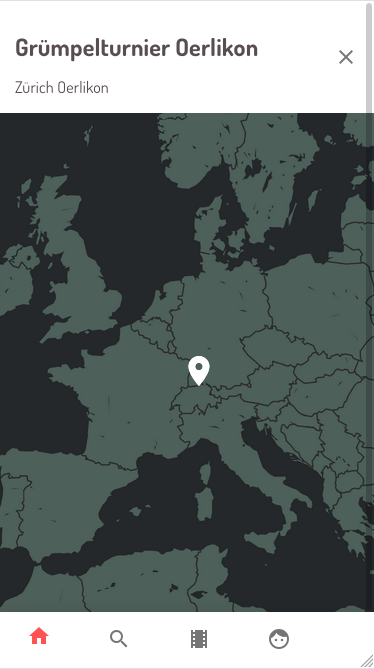
\includegraphics[width=7cm]{images/map.png}
    \caption{Event Map \protect\footnotemark}
    \label{img:event-map}
\end{figure}
In the second tab of the application, all events are displayed in a conventional list format \ref{img:event-list}. Here they can be filtered through a search bar, which performs a full text search on all the event properties. This enables searches by various properties such as location, title, and type all through the same search field.

\begin{figure}[H]
    \centering
    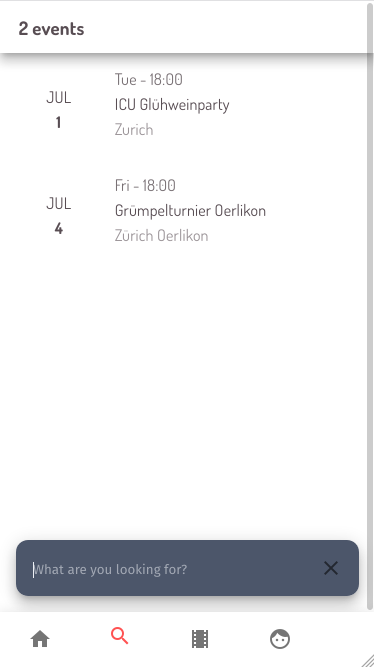
\includegraphics[width=7cm]{images/event_list.png}
    \caption{Event list}
    \label{img:event-list}
\end{figure}

When a user selects an event through one of the aforementioned views, he is taken to the event detail \ref{img:event-details} page. This is the most information-rich view of the application, since it contains most of the SC interaction possibilities. First presented is all of the information on the event, as well as the identity approver chosen by the event host, if any. Further down, the user can see a graphical representation of all ticket categories. The user can buy any of the available tickets by tapping on the desired category/seat and submitting the appearing pop-up. If the event is still in its \textit{presale phase}, the user can also join the presale from within this view. 
\begin{figure}[!tbp]
  \centering
  \subfloat[Event Information]{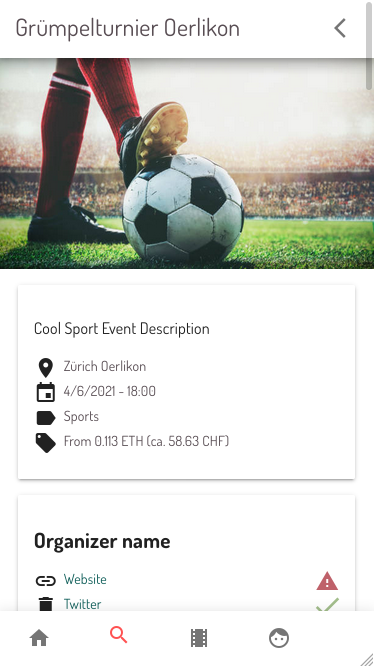
\includegraphics[width=0.3\textwidth]{images/event_1.png}\label{fig:f1}}
  \hfill
  \subfloat[Seating Plan]{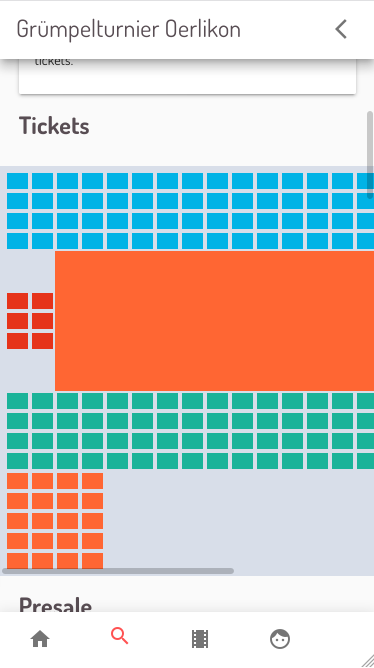
\includegraphics[width=0.3\textwidth]{images/event_2.png}\label{fig:f2}}
    \hfill
    \subfloat[Aftermarket]{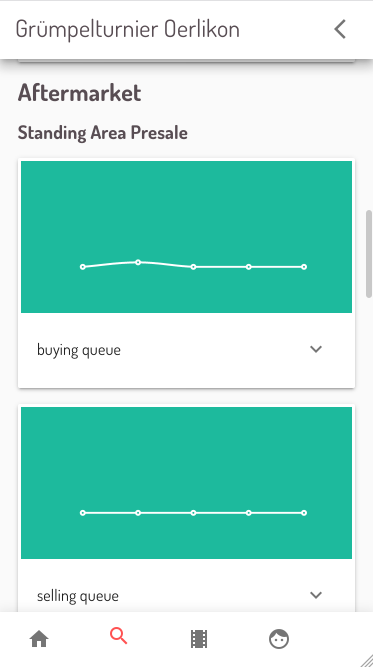
\includegraphics[width=0.3\textwidth]{images/event_3.png}\label{fig:f3}}

  \caption{Event Detail View}
  \label{img:event-details}
\end{figure}
Lastly, the aftermarket state is shown for each ticket category. This is done via line graphs, showing each queue as described in \ref{section:aftermarket}. For the \textit{buying queues}, the user can directly enqueue or buy an aftermarket ticket if there are offerings in the selling queue. The selling queues can be joined from the inventory view, as described later on in this section.

The third section of the application displays the tickets bought by the user and joined presales. For each ticket, the user can open a modal content window, showing all relevant ticket information by clicking on the ticket. In addition to all information regarding the event and the specific ticket, the user can also choose to sell his ticket from this view.
\begin{figure}[!tbp]
  \centering
  \subfloat[Ticket List]{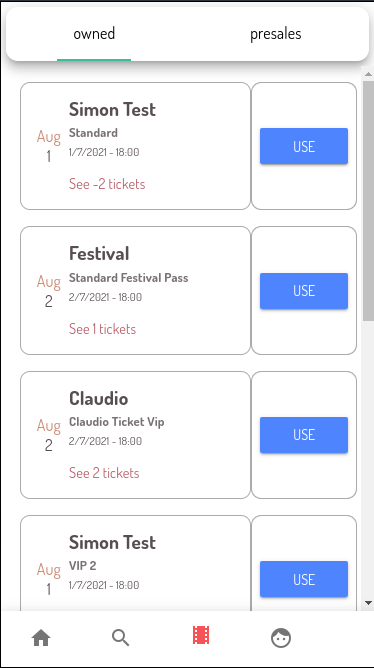
\includegraphics[width=0.4\textwidth]{images/in_1.png}\label{fig:f1}}
  \hfill
  \subfloat[Ticket Details]{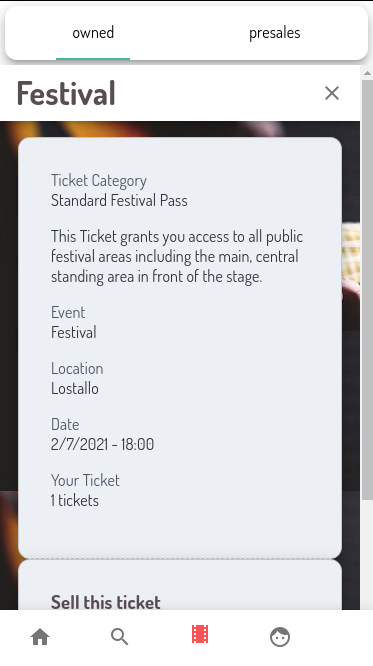
\includegraphics[width=0.4\textwidth]{images/in_2.png}\label{fig:f2}}
  \caption{Inventory view}
  \label{img:inventory}
\end{figure}

In the last tab, information regarding the identity approval status with all registered identity approvers is shown to the user . For each approver, the levels of authentication are displayed in increasing order of severity, as well as the users current level of authentication. Since each event can use any registered third party as approval service, there might exist identity approvers with their own, external approval services. For these, the user has to inform himself via the information provided by the respective event host on how to reach the necessary level of authentication. \\
If an event host has chosen the \textit{Idetix Identity Approver} for his event, the user can complete the approval process from within the application. This is done via one of the methods described in [Ref]. 
\begin{figure}[H]
    \centering
    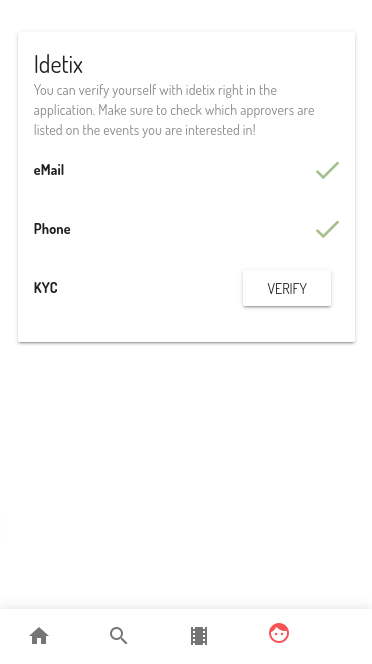
\includegraphics[width=7cm]{images/ide_1.png}
    \caption{Identity approval view}
    \label{img:identity}
\end{figure}

